\documentclass[aspectratio=169]{beamer}
\beamertemplatenavigationsymbolsempty
%\setbeameroption{show only notes}
%\setbeameroption{show notes on second screen}

\usepackage{graphicx}
\graphicspath{{figures}{figures/graphics}}

\usepackage[]{xcolor}

\usepackage{tikz}
\usepackage{tikzscale}
\usetikzlibrary{shapes, arrows.meta, positioning, calc, intersections}
\tikzstyle{block} = [rectangle, draw, rounded corners]


\usepackage[export]{adjustbox}

\usepackage{caption}
\captionsetup[figure]{labelformat=empty, font=tiny, labelfont=scriptsize}

\usepackage{subcaption}
\usepackage{multicol}
\usepackage{bm}
\usepackage{booktabs}


%\usepackage[numbers, sort&compress]{natbib}
%\bibliographystyle{abbrvnat}

\usepackage[style=authoryear]{biblatex}
\addbibresource{bibliography.bib}


% selectively hide table columns
\usepackage{array}
\newcolumntype{H}{>{\setbox0=\hbox\bgroup}c<{\egroup}@{}}


% beamer style
\setbeamertemplate{blocks}[rounded][shadow]
\setbeamercolor{block body}{bg=structure!10}
\setbeamercolor{block title}{bg=structure!20}

\setbeamercolor{block body example}{bg=green!10}
\setbeamercolor{block title example}{bg=green!20}

\setbeamercolor{block body alerted}{bg=red!10}
\setbeamercolor{block title alerted}{bg=red!20, fg=black}

\input{includes/uvmcolors.tex}
\title{Smoking Reduction Trajectories and their Associations with Smoking Cessation}
\subtitle[]{VCBH Retreat}
%%%%%
\author[]{Anthony Barrows$^{1,2}$, Elias Klemperer$^{1,3}$, Hugh Garavan$^{1}$, Nicholas Allgaier$^{1,2}$, Nicola Lindson$^4$, Gemma Taylor$^5$}
%\date{\today}
\institute{
	$^1$ 
\includegraphics[width=.75in]{uvm}
	$^2$ \includegraphics[width=.75in]{complexsystems}
	$^3$ 
\includegraphics[width=.75in]{vcbh}
	$^4$ \includegraphics[width=.75in]{oxford_logo}
	$^5$ \includegraphics[width=.75in]{bath_logo}
}
\date{}

\makeatletter
\newcommand\insertlogoi[2][]{\def\@insertlogoi{\includegraphics[#1]{#2}}}
\newcommand\insertlogoii[2][]{\def\@insertlogoii{\includegraphics[#1]{#2}}}
\newlength\LogoSep
\setlength\LogoSep{0pt}
\makeatother

% defined colors

\definecolor{class1}{HTML}{F8766D}
\definecolor{class2}{HTML}{7CAE00}
\definecolor{class3}{HTML}{00BFC4}

% just have frame number in footline
\setbeamertemplate{footline}[frame number]

\def\swidth{2cm}
\usetheme[width=\swidth]{Hannover}
%\usecolortheme{spruce}

%\usecolortheme{}

%%%%% ADD  NOPHOTO Icon

%
%\makeatletter
%\addtobeamertemplate{sidebar left}{}{%
%	\begin{minipage}{\swidth}
%		\centering
%		\includegraphics[width=0.3\textwidth]{../../../pres-images/no-photo}
%	\end{minipage}
%	
%
%}
%\makeatother


% numberless footnote
\newcommand\blfootnote[1]{%
	\begingroup
	\renewcommand\thefootnote{}\footnote{#1}%
	\addtocounter{footnote}{-1}%
	\endgroup
}

% remove citation numbers from footnotes, too
\makeatletter
\def\@makefnmark{}
\makeatletter

% in-press/inprep citaiton command
\newcommand{\reviewcite}{\blfootnote{\tiny Barrows et al., \textit{In review}}}

% for inserting tiny papers
\newcommand{\smallpaperwidth}{0.175}

% co-authors' images

\newcommand{\coauthorimg}[3]{%
	\begin{minipage}{0.16\textwidth}
		\begin{figure}
				\begin{minipage}{\linewidth}
					\includegraphics[width=\linewidth]{#1}
					\caption{#2 \\ #3}
					%			\caption{#3}
				\end{minipage}
		\end{figure}
	\end{minipage}

}
\newcommand{\smallimagewidth}{0.15\textwidth}

\begin{document}
	
	\begin{frame}
		\maketitle
		\note{Mention data science/machine learning approach.}
	\end{frame}

	
	%% Outline
%\begin{frame}{Outline}
%	\tableofcontents
%\end{frame}

%\begin{frame}{Paper}
%		\begin{columns}
%		\column{0.2\textwidth}
%		\includegraphics[width=\columnwidth]{papers/Marek22}
%		\column{0.8\textwidth}
%		\href{https://www.nature.com/articles/s41586-022-04492-9}{Reproducible brain-wide association studies require thousands of individuals \footcite{MarekEtAl2022}}
%
%		Reasons:
%		\begin{itemize}
%			\item
%		\end{itemize}
%	\end{columns}
%\end{frame}


\begin{frame}{Disclosures}
	This work is supported by:
	\begin{columns}
		\begin{column}{0.75\textwidth}
			\begin{itemize}
				\small
				\item  NIDA T32DA045593
				\item NIGMS P20GM103644
				\item Cancer Research UK (PRCPJT-Nov22/100012, PPRCPJT\textbackslash100,023, and C56067/A21330)
				\item The University of Oxford and  NHS Greater Manchester Integrated Care
			\end{itemize}

		\end{column}
		\begin{column}{0.25\textwidth}
			\includegraphics[width=\columnwidth]{complexbrain}
		\end{column}
	\end{columns}
	
	\vspace{1em}
	
	\begin{itemize}
		\scriptsize
		\item 	Gemma Taylor works for a scientific consulting company offering statistical services for projects unrelated to this research.
		\item The current authors were not involved in the design, conduct, analysis, write-up or dissemination of the original trials, and the funder of these trials (McNeil AB) had no involvement in the planning, analysis, or interpretation of this secondary analysis.
	\end{itemize}

	
	
\end{frame}
\section{Introduction}

\begin{frame}{Introduction}
	\begin{itemize}

		\item Smoking is the leading cause of premature death and preventable illness worldwide \footcite{worldhealthorganizationWHOReportGlobal2011}.
		\pause
		\item Treatment is often designed for people motivated to quit now, but many are not \footcite{ReidEtAl2019, WewersEtAl2003}
		\pause
		\item A common suggestion is smoking reduction.

	\end{itemize}
\end{frame}



\begin{frame}{Introduction}
		\begin{columns}
			\column{0.3\textwidth}
			\includegraphics[width=\columnwidth]{lindson19}
			\footcite{lindsonSmokingReductionInterventions2019}
			\column{0.7\textwidth}
	
			However $\ldots$
			\vspace{5mm}
		
			\begin{itemize}
				\item A prior Cochrane review found that reduction interventions are no more or less effective than quitting abruptly.
				\pause
				\item Little is known about how people reduce their smoking and which smoking reduction patterns predict better cessation outcomes.
				\begin{itemize}
					\item Many ways to reduce 
					\item What is the best way?
				\end{itemize}
			\end{itemize}
		\end{columns}
\end{frame}

%
\begin{frame}{Introduction}
	\begin{block}{}
		\begin{itemize}
			 \raggedright
			\item When people (who are not motivated to quit) are asked to reduce smoking, how do people choose to do so? 
			\pause
			\item Are there smoking or demographics associated with certain reduction patterns?
			\pause
			\item Which patterns of reduction are associated with better cessation outcomes?
		\end{itemize}
	\end{block}
	
	

\end{frame}

\section{Methods}
\subsection{Data}

\begin{frame}{Methods}
	Combine data from 5 RCTs of nicotine replacement therapy (NRT) in people not looking to quit smoking (the ``McNeil Trials'') \footcite{wennikeSmokingReductionPromotes2003,rennardEfficacyNicotineInhaler2006,bolligerSmokingReductionOral2000,batraSmokingReductionTreatment2005,hausteinDoubleblindRandomizedPlacebocontrolled2001}:
	
	\begin{itemize}
		\item<1-> Baseline and follow-up (weeks 2, 10, 18, and 26) CPD
		\item<2-> Measures of anxiety, depression, and nicotine dependence
		\item<3-> Biochemically-verified smoking cessation at week 52
	\end{itemize}	
	
	\visible<1->{%
			\centering
		\includegraphics[width=\smallpaperwidth\textwidth]{batra05}
		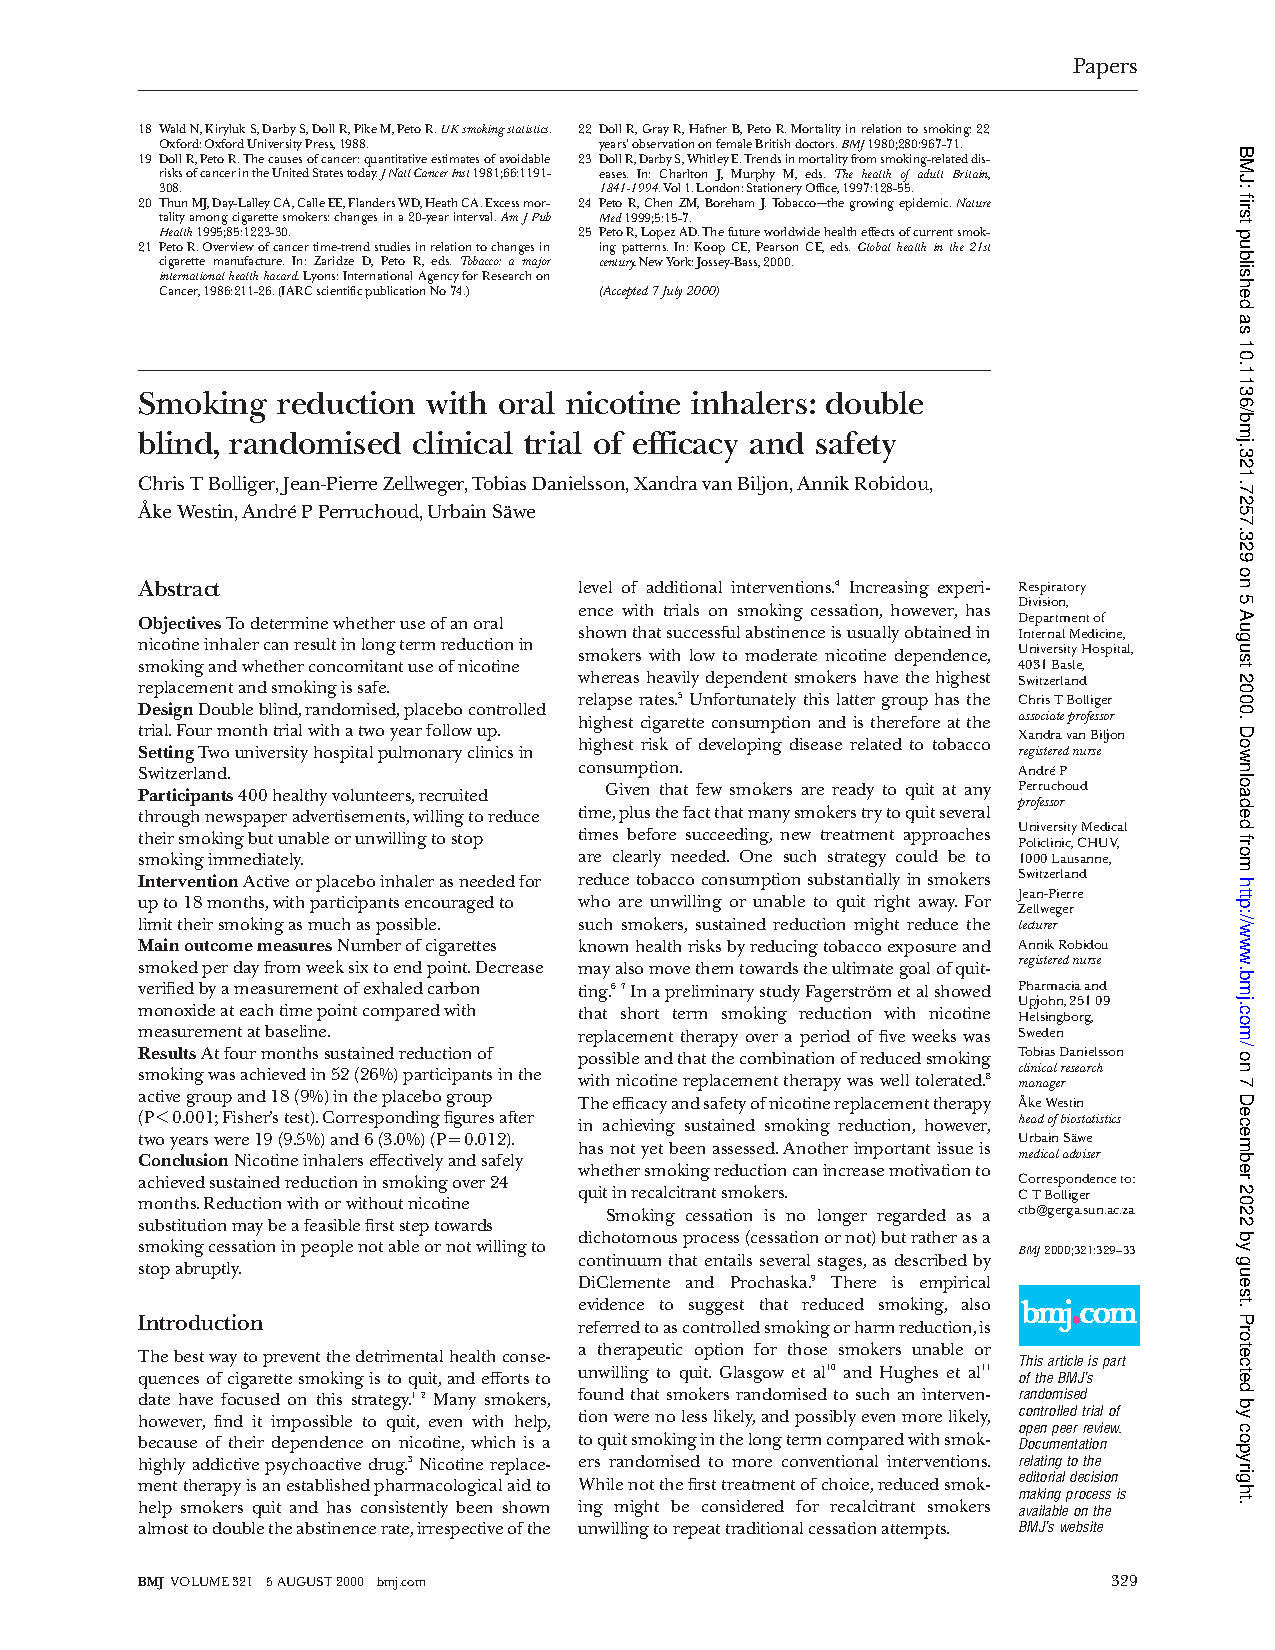
\includegraphics[width=\smallpaperwidth\textwidth]{bolliger00}
		\includegraphics[width=\smallpaperwidth\textwidth]{haustein01}
		\includegraphics[width=\smallpaperwidth\textwidth]{rennard06}
		\includegraphics[width=\smallpaperwidth\textwidth]{wennike03}
	}

	

\end{frame}

\begin{frame}{Methods}
		Participants in each of the included trials were:
		\begin{itemize}
		\item enrolled if they 
		\begin{itemize}
			\item smoked $\geq 15$ CPD
			\pause
			\item made a serious quit attempt within the past 2 years 
			\pause
			\item were currently unmotivated to quit
			\pause
			\note{Details about motivation weren't reported}
			\item wanted to reduce their smoking using NRT
		\end{itemize}
		\pause
		\item randomly assigned to receive active or placebo NRT 
		\pause
		\item were told to reduce their smoking as much as possible
		\note{Each study reported that participants were ``provided with information on possible ways to'' reduce their smoking.}

	\end{itemize}
		\vspace{2cm}
		\fbox{\begin{minipage}{\linewidth}
			\small
			\begin{itemize}
				\item Pre-registered protocol: \texttt{https://osf.io/qh378/}
				\item Analytical code: \texttt{https://github.com/ajbarrows/mcneil-lca}
			\end{itemize}
	\end{minipage}}
\end{frame}

	
\subsection{Analysis}

\begin{frame}{Analysis}


\centering
\includegraphics[width=0.9\textwidth]{overview}

\end{frame}

\begin{frame}{Analysis}
	\begin{columns}
		\column{0.4\textwidth}
		\textbf{Baseline Variables} \\
		\vspace{2mm}
		\begin{tiny}
			Demographics
			\begin{itemize}
				\item Age
				\item Sex
			\end{itemize}
			Parent Trial Information
			\begin{itemize}
				\item Study site
				\item Treatment group
			\end{itemize}
			Mental and Physical Health
			\begin{itemize}
				\item SCQoL Anxiety, Depression
				\item SF-36 Sub Scales
			\end{itemize}
			Smoking Characteristics
			\begin{itemize}
				\item Age started smoking
				\item CO
				\item CPD
				\item FTND
				\item Intention to quit
				\item Last cigarette experience
				\item Longest period without smoking
				\item Number of quit attempts
				\item Time since last quit attempt
			\end{itemize}
		\end{tiny}

		\column{0.6\textwidth}
			\includegraphics[width=\columnwidth]{overview2_limited}
	\end{columns}

\end{frame}


\begin{frame}{Analysis}
	
	
	\centering
	\includegraphics[width=0.9\textwidth]{overview}
	
\end{frame}

\section{Results}
\subsection{Participants}

\begin{frame}{Results}
	\framesubtitle{Participants}
	
	\begin{columns}
		\column{0.4\textwidth}
				\scalebox{.6}{%
				\centering
	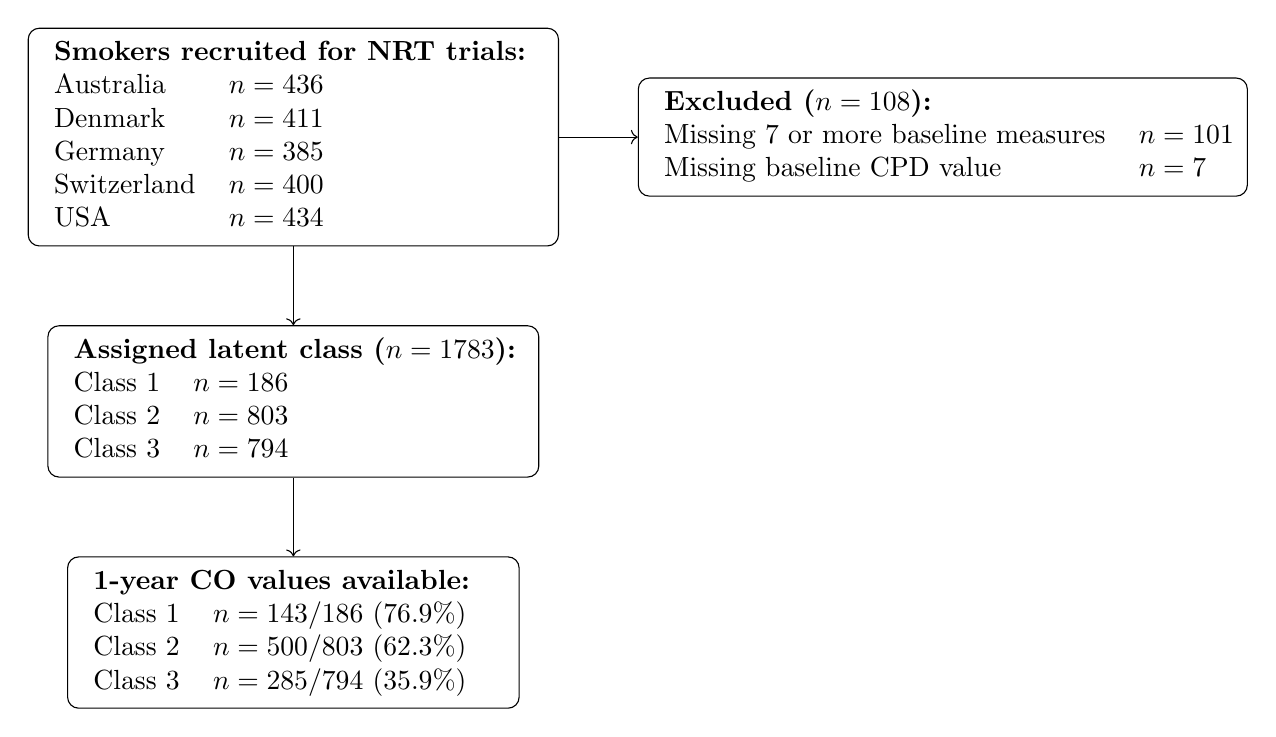
\begin{tikzpicture}[auto]
		\node [block] (init) {
			\parbox{6.5 cm}{
				\begin{tabular}{ll}
					\multicolumn{2}{l}{{\textbf{Smokers recruited for NRT trials:}}} \\
					Australia & $n = 436$ \\
					Denmark & $n = 411$ \\
					Germany & $n = 385$ \\
					Switzerland & $n = 400$ \\
					USA & $n = 434$
				\end{tabular}
				
			}
		};
		
		\node[block, right=of init] (excluded) {
			\parbox{7.5cm}{
				\begin{tabular}{ll}
					\multicolumn{2}{l}{{\textbf{Excluded ($n = 108$):}}} \\
					Missing 7 or more baseline measures & $n = 101$ \\
					Missing baseline CPD value & $n = 7$
			\end{tabular}
		}
		};
		
		\node [block, below= of init] (lca) {
			\parbox{6cm}{
				\begin{tabular}{ll}
					\multicolumn{2}{l}{{\textbf{Assigned latent class ($n = 1783$):}}} \\
					Class 1& $n = 186$ \\
					Class 2 & $n = 803$ \\
					Class 3 & $n = 794$
			\end{tabular}
		}
		};
		\node [block, below = of lca] (co) {
			\parbox{5.5cm}{
				\begin{tabular}{ll}
					\multicolumn{2}{l}{{\textbf{1-year CO values available:}}} \\
					Class 1& $n = 143/186$ (76.9\%)\\
					Class 2 & $n = 500/803$ (62.3\%) \\
					Class 3 &  $n = 285/794$ (35.9\%)
				\end{tabular}
				
		}};
		
		\draw[->] (init.east) -- (excluded.west);
		\draw[->] (init.south) -- (lca.north);
		\draw[->] (lca.south) --(co.north);
		
	\end{tikzpicture}

		}
		
		\note{Rather than introduce more bias through imputation, we opted for list-wise deletion.}
		\column{0.4\textwidth}
		
				\begin{tiny}
				\begin{tabular}{llHHH}
					\toprule
					& Overall & Class 1       & Class 2       & Class 3       \\
					\cmidrule{2-5}
					N (\%)                         & 1783 (100)      & 186 (10.4)    & 803 (45.0)    & 794 (44.5)    \\
					\midrule
					Study Site (\%)                &                 &               &               &               \\
					\hspace{3mm}Australia                      & 360 (20.2)      & 32 (17.2)     & 159 (19.8)    & 169 (21.3)    \\
					\hspace{3mm}Denmark                        & 340 (19.1)      & 35 (18.8)     & 175 (21.8)    & 130 (16.4)    \\
					\hspace{3mm}Germany                        & 353 (19.8)      & 60 (32.3)     & 153 (19.1)    & 140 (17.6)    \\
					\hspace{3mm}Switzerland                    & 301 (16.9)      & 29 (15.6)     & 139 (17.3)    & 133 (16.8)    \\
					\hspace{3mm}USA                            & 429 (24.1)      & 30 (16.1)     & 177 (22.0)    & 222 (28.0)    \\
					Active NRT (\%) & 900 (50.5)      & 125 (67.2)    & 413 (51.4)    & 362 (45.6)    \\
					Sex = Male (\%)                & 798 (44.8)      & 96 (51.6)     & 357 (44.5)    & 345 (43.5)    \\
					Age (m(sd))                & 44.10(10.72)    & 45.79 (11.41) & 44.26 (10.52) & 43.53 (10.73) \\
					FTND (m(sd))      & 6.14 (2.00)     & 5.60 (2.13)   & 6.11 (2.01)   & 6.30 (1.94)   \\
					CPD (m(sd))       & 27.32 (9.73)    & 25.65 (10.37) & 27.42 (9.78)  & 27.62 (9.50)  \\
					SCQoL Anxiety (m(sd))              & 0.45 (0.85)     & 0.41 (0.83)   & 0.41 (0.82)   & 0.51 (0.90)   \\
					SCQoL Depression (m(sd))       & 0.29 (0.69)     & 0.29 (0.69)   & 0.26 (0.67)   & 0.32 (0.71) \\
					\bottomrule
				\end{tabular}
				\end{tiny}

				
				\begin{center}
					\begin{minipage}{\columnwidth}
						\begin{itemize}
							\raggedright
							\tiny
							\item 	1053 (59.1\%) were enrolled in trial that used NRT gum
							\item 	n=730 (40.9\%) used inhalers
						\end{itemize}
					\end{minipage}
				\end{center}



		


	\end{columns}

\end{frame}



\subsection{Latent Class Analysis}
\begin{frame}{Results}
	\framesubtitle{Latent Class Analysis}
	\includegraphics[width=0.75\textwidth]{overview1}
%	\vspace{3cm}
	\centering
	\includegraphics[width=0.4\textwidth]{pres/bic_pres}
\end{frame}


\begin{frame}{Results}
	\note{Start by orienting to the graph}
	\framesubtitle{Latent Class Analysis}
	\begin{columns}
		\column{0.6\textwidth}
			\includegraphics[width=\columnwidth]{smoking_traj}
		\column{0.4\textwidth}
			\begin{itemize}
				\small
				\item \textcolor{class1}{Class 1 (substantial reducers):} 10.43\% initially reduced and nearly eliminated smoking
				\item \textcolor{class2}{Class 2 (moderate reducers):} 45.04\% reduced by nearly 50\% and remained
				\item \textcolor{class3}{Class 3 (minimal reducers):} 44.53\% initially reduced but reverted to their baseline smoking
			\end{itemize}
	\end{columns}

\reviewcite

\end{frame}


\subsection{Predicting Latent Class}

\begin{frame}{Results}
	\framesubtitle{Predicting Latent Class}
	\centering
	\includegraphics[width=0.8\textwidth]{overview2}
	\begin{columns}
		\column{0.5\textwidth}
		\begin{itemize}
			\small
			\item Dataset initially divided into 80\% training and 20\% testing partitions
			\item 5-fold cross-validation performed with training set
			\begin{itemize}
				\item Each fold further divided into 5 ``inner folds'' for selecting optimal hyperparameters
			\end{itemize}
		\end{itemize}
			
		\column{0.5\textwidth}
		\includegraphics[width=.8\columnwidth]{crossval_diagram}
	\end{columns}

\end{frame}


\begin{frame}{Results}
	\framesubtitle{Predicting Latent Class}
	Predictive performance assessed using unseen data (i.e.,  20\% held-out testing partition)
	\begin{columns}
		\column{0.35\textwidth}
		\includegraphics[width=\columnwidth]{lca_roc}
		\column{0.65\textwidth}
		\begin{itemize}
			\scriptsize
			\item \textcolor{class1}{substantial reducers (Class 1)} test AUC = 0.766, $p<.001$
			\item \textcolor{class2}{moderate reducers (Class 2)} test AUC = 0.569, $p=.008$ 
			\item \textcolor{class3}{minimal reducers (Class 3)} test AUC = 0.523, $p<.001$ 
		\end{itemize}
		
		\vspace{1cm}
		
		\begin{center}
				\fbox{\begin{minipage}{0.5\columnwidth}
				\tiny
				Note: 		
				Statistical significance determined with respect to $ROC AUC=0.5$ and concordance its with the Mann-Whitney $U$ statistic:
				\begin{equation*}
					AUC = \frac{U}{n_1n_2}
				\end{equation*}
		\end{minipage}}
		\end{center}
	\end{columns}
	\reviewcite

\end{frame}

\begin{frame}{\tiny Results}
%	\framesubtitle{Predicting Latent Class}
	\begin{columns}
		\column{0.85\textwidth}
			\includegraphics[width=\columnwidth]{pres/fis_lca_justclass_pres}
	
		\column{0.15\textwidth}

		\begin{itemize}
				\tiny
%			\item \textcolor{class1}{substantial reducers (Class 1): }Tended to be older with lower anxiety and nicotine dependence, more likely to have received active NRT.
			\item \textcolor{class1}{substantial reducers (Class 1): } Older, anxiety  + FTND $\downarrow$
			\item \textcolor{class2}{moderate reducers (Class 2): }No clear pattern
			\item \textcolor{class3}{minimal reducers (Class 3): }Inverse of \textcolor{class1}{Class 1}
		\end{itemize}
		
		\vspace{2mm}
		\includegraphics[width=\columnwidth]{smoking_traj_notitle}

	\end{columns}
	\reviewcite

\end{frame}



%
\subsection{Predicting Smoking Cessation}

\begin{frame}{Results}
	\framesubtitle{Predicting Smoking Cessation}
	\includegraphics[width=\textwidth]{overview3}
\end{frame}

\begin{frame}{Results}
	\framesubtitle{Predicting Smoking Cessation}
		\begin{center}
			\scalebox{.7}{%
				%\documentclass[]{article}
%\usepackage{fullpage}
%
%\usepackage{tikz}
%\usetikzlibrary{shapes, arrows, positioning}
%\tikzstyle{block} = [rectangle, draw, rounded corners]
%
%%opening
%%\title{}
%%\author{}
%\date{}
%\begin{document}

%\begin{figure}
%	\centering
	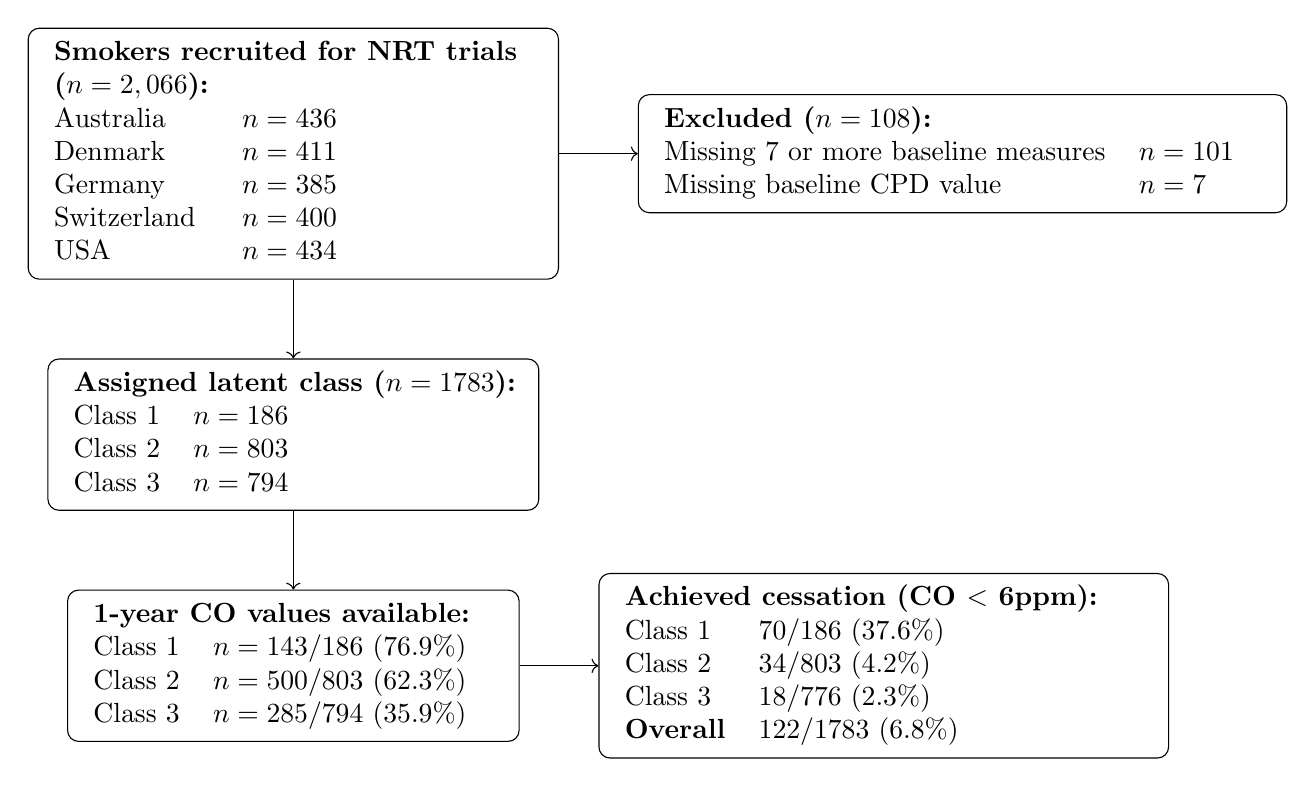
\begin{tikzpicture}[auto]
		\node [block] (init) {
			\parbox{6.5 cm}{
				\begin{tabular}{ll}
					\multicolumn{2}{l}{{\textbf{Smokers recruited for NRT trials}}} \\
					 \textbf{($n=2,066$):} \\
					Australia & $n = 436$ \\
					Denmark & $n = 411$ \\
					Germany & $n = 385$ \\
					Switzerland & $n = 400$ \\
					USA & $n = 434$
				\end{tabular}
				
			}
		};
		
		\node[block, right=of init] (excluded) {
			\parbox{8cm}{
				\begin{tabular}{ll}
					\multicolumn{2}{l}{{\textbf{Excluded ($n = 108$):}}} \\
					Missing 7 or more baseline measures & $n = 101$ \\
					Missing baseline CPD value & $n = 7$
			\end{tabular}
		}
		};
		
		\node [block, below= of init] (lca) {
			\parbox{6cm}{
				\begin{tabular}{ll}
					\multicolumn{2}{l}{{\textbf{Assigned latent class ($n = 1783$):}}} \\
					Class 1& $n = 186$ \\
					Class 2 & $n = 803$ \\
					Class 3 & $n = 794$
			\end{tabular}
		}
		};
		\node [block, below = of lca] (co) {
			\parbox{5.5cm}{
				\begin{tabular}{ll}
					\multicolumn{2}{l}{{\textbf{1-year CO values available:}}} \\
					Class 1& $n = 143/186$ (76.9\%)\\
					Class 2 & $n = 500/803$ (62.3\%) \\
					Class 3 &  $n = 285/794$ (35.9\%)
				\end{tabular}
				
		}};
	
		\node[block, right = of co] (quit) {
			\parbox{7cm}{
			\begin{tabular}{ll}
				\multicolumn{2}{l}{{\textbf{Achieved cessation (CO $<$ 6ppm):}}} \\
				Class 1 & 70/186 (37.6\%) \\
			Class 2 & 34/803 (4.2\%) \\
			Class 3 & 18/776 (2.3\%) \\
			\textbf{Overall} & 122/1783 (6.8\%)
			\end{tabular}
		

				
			}
		};

		
		\draw[->] (init.east) -- node[auto, shorten >=5pt] {} (excluded.west);
		\draw[->] (init.south) -- node[above=10mm] {} (lca.north);
		\draw[->] (lca.south) --node[above=10mm] {} (co.north);
		\draw[->] (co.east) --node[left=10mm] {} (quit.west);
		
	\end{tikzpicture}
%	\caption{Participant record availability flowchart.}
%	\label{fig:flowchart}
%\end{figure}
%\end{document}

			}
	\end{center}
\end{frame}

\begin{frame}{Results}
		\framesubtitle{Predicting Smoking Cessation}
		\begin{columns}
			\column{0.45\textwidth}
			\includegraphics[width=\columnwidth]{quit_roc}
			\column{0.55\textwidth}
				
				 Elastic net logistic regression predicting smoking cessation using
				\begin{itemize}
					\scriptsize
					\item baseline characteristics alone: \\ AUC = $0.632 \pm 0.006$, $p<.001$
					\item baseline characteristics plus latent class: AUC = $0.776 \pm 0.010$, $p<.001$
				\end{itemize}
				\begin{block}{}
					Adding latent class as an independent variable improved cessation prediction by 14.4\%
				\end{block}
		\end{columns}
		\reviewcite
\end{frame}



\section{Conclusion}

\begin{frame}{Conclusions}
	\begin{columns}
		\column{0.6\textwidth}
		\begin{itemize}
			\item<1-> Examining latent trajectories in smoking behavior among people not motivated to quit revealed three distinct patterns
			\item<2-> Those who reduced their smoking by $\geq 50\%$ in the first two weeks were more than twice as likely to quit
			\item <3-> First study to date to use rigorous machine learning-based methods to predict latent smoking reduction behavior
		\end{itemize}
		\column{0.4\textwidth}
		\visible{%
						\includegraphics[width=\columnwidth]{smoking_traj}
		}

	\end{columns}
\end{frame}

% limitations



% TODO add pauses

\begin{frame}{Conclusion}
	\framesubtitle{Clinical Implications}
	\begin{itemize}
		\item Lots of early reduction is most likely to encourage cessation
			\pause
		\item 50\% reduction is often considered the threshold for successful smoking reduction
		\begin{itemize}
			\item We validate this analytically
		\end{itemize}
			\pause
		\item Not all reduction interventions are equally likely to result in cessation
	
	\end{itemize}
\end{frame}
% (unsurprisingly) we found that we need to generate a lot of early reduction to encourage quitting
% comon threshold is 50% cutoff to bifurcate whether somoene reproduced or not. we validate this analytically
% need to take caution when collapsing across reduction interventions (e..g, not push people too hard, low hanging fruit)

% TODO ADD LIMITATIONS

% include limitations/strengths if time

\begin{frame}{Thank You}
%	\includegraphics[width=\smallimagewidth]{people/eli}
%	\includegraphics[width=\smallimagewidth]{people/hugh}
%	\includegraphics[width=\smallimagewidth]{people/nick}
%	\includegraphics[width=\smallimagewidth]{people/nicola}
%	\includegraphics[width=\smallimagewidth]{people/gemma}
%
\centering
\begin{tabular}{ccccc}
	\coauthorimg{people/eli}{Eli Klemperer, PhD}{University of Vermont} &
	\coauthorimg{people/hugh}{Hugh Garavan, PhD}{University of Vermont} &
	\coauthorimg{people/nick}{Nick Allgaier, PhD}{University of Vermont} &
	\coauthorimg{people/nicola}{Nicola Lindson, PhD}{University of Oxford} &
	\coauthorimg{people/gemma}{Gemma Taylor, PhD}{University of Bath} 
\end{tabular}

\centering
\includegraphics[width=1in]{complexbrain}

\includegraphics[width=2in]{vcbh}

\end{frame}



\begin{frame}[allowframebreaks]{References}

		\tiny
		\printbibliography

\end{frame}

\begin{frame}{}
%	\framesubtitle{Feature Importance}
	
		\includegraphics[width=0.9\textwidth]{pres/fis_lca_pres}
	\reviewcite
\end{frame}

\begin{frame}{}
	\includegraphics[width=0.75\textwidth]{pres/fis_cessation_pres}
	\reviewcite
\end{frame}

	
	
\end{document}


